% Copyright 2009--2010  Ed Bueler

\section{next steps}

\subsection{practicalities}

\begin{frame}[fragile]
\frametitle{what technical skills are needed for \\ numerical ice sheet modeling?}

you need:

\begin{itemize}
\item comfort in a technical computing environment, usually Unix, in which you need to know:
  \begin{itemize}\small
  \item[$\circ$] an editor,
  \item[$\circ$] a compiled language (Fortran or C),
  \item[$\circ$] a scripting/prototyping language (Matlab, Python, etc.), and
  \item[$\circ$] \emph{a version control system} (Subversion, git, etc.)
  \normalsize
  \end{itemize}
\item willingness to read math, numerical analysis, computer science books
\item \dots and willingness to ignor \emph{some} of the advice found there
\item know some tools for NetCDF files
\item get exposed to parallel computing
\item but, at the end of the day: \emph{physics}
\end{itemize}
\end{frame}


\begin{frame}
\frametitle{what technical skills are needed? 2}

\begin{itemize}
\item an important skill is to \emph{not} re-invent the wheel
\item \emph{never} re-invent the wheel for basic numerics:
  \begin{itemize}
  \item[$\circ$] \Matlab, Comsol, PETSc, libmesh, Elmer, Trilinos, Triangle, etc.~handle fundamental numerical linear algebra, mesh generation, finite element assembly and solve, etc.~tasks; don't even try to compete!
  \item[$\circ$] \dots except to write throw-away codes to help you \emph{understand} numerical ideas 
  \end{itemize}
\item sometimes there is no need to re-invent ice sheet modeling:
  \begin{itemize}
  \item[$\circ$] open source SIA-based comprehensive models: GLIMMER, SICOPOLIS
  \item[$\circ$] open source hybrid/higher-order/Stokes models: PISM, Elmer-ice, CISM
  \end{itemize}
\item glacier and ice sheet modeling is young!  there is much to do!
\end{itemize}
\end{frame}


\subsection{omitted models}

\begin{frame}{omitted models 1: thermomechanical coupling}

\begin{columns}
\begin{column}{0.6\textwidth}
\begin{itemize}
\item the softness of ice ``$A$'' is not constant!
  \begin{itemize}
  \item[$\circ$] $A=A(T)$ varies by more than $10^3$ in the $50\phantom{|}^\circ\text{C}$ ice temperature range relevant to Antarctic ice
  \item[$\circ$] dissipation of flow energy is significant in conservation of energy equation
  \item[$\circ$] \dots and there is a ``new'' fluid instability from feedback between the above two items \scriptsize (lower figure; EISMINT II [Payne and others, 2000]\nocite{EISMINT00}) \small
  \end{itemize}
\item ice temperature is part of the ``long memory'' of the ice sheets for past climate
\item conservation of energy is just as important for fast scale dynamics (involving sliding and hydrology) as it is for ``long memory'' questions
\end{itemize}
\end{column}
\begin{column}{0.4\textwidth}
\vspace{-0.2in}
  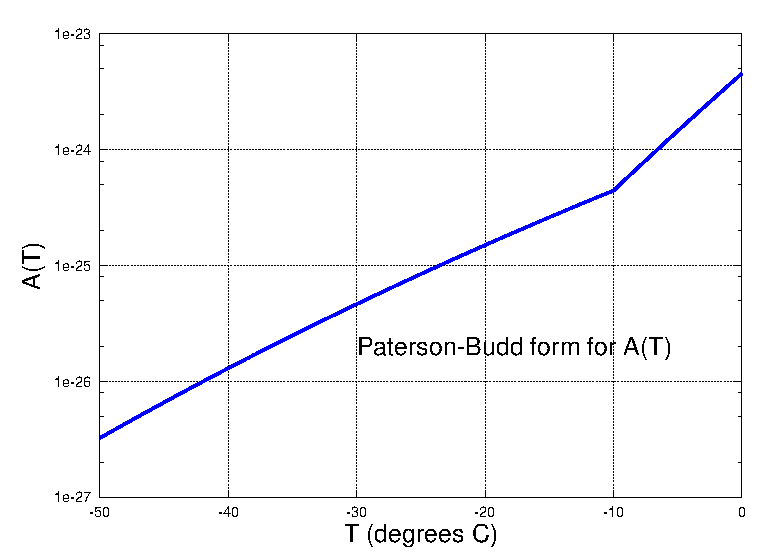
\includegraphics[width=1.0\textwidth]{pdffigs/AofT}
  
\bigskip
  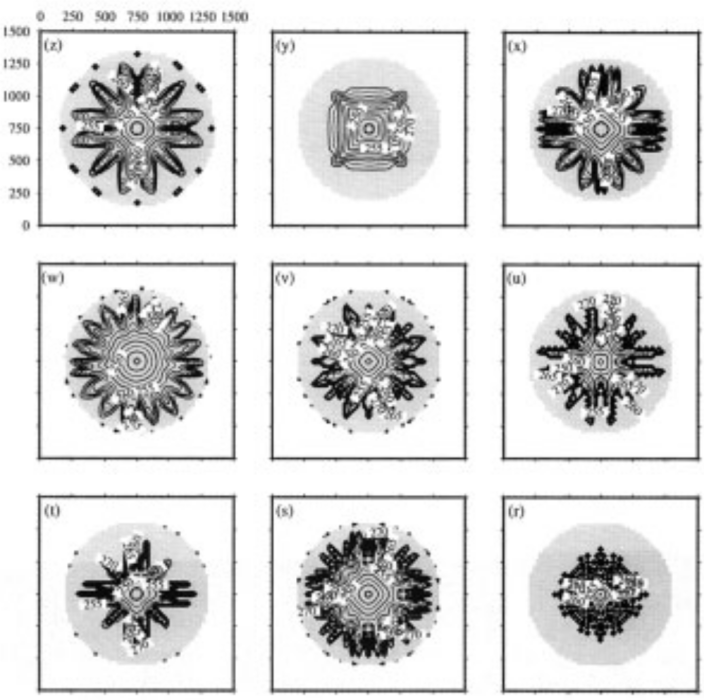
\includegraphics[width=1.0\textwidth]{photos/eisIIF}
\end{column}
\end{columns}
\end{frame}


\begin{frame}{omitted models 2: surface mass balance}

\begin{itemize}
\item ice sheet models need \emph{modeled} surface mass balance
  \begin{itemize}
  \item[$\circ$] over paleoglacial time scales
  \item[$\circ$] and when modeling response to future changes
  \end{itemize}
\item models include:
  \begin{itemize}
  \item[$\circ$] positive degree-day (PDD) and other index models
  \item[$\circ$] energy-balance models
  \end{itemize}
\nocite{Hock05}
%\item read: [Hock, 2005]\nocite{Hock05} $=$ survey of observations and processes
\item very significant source of uncertainty for Greenland ice sheet dynamics!
\end{itemize}
\end{frame}


\begin{frame}{omitted models 3: solid Earth deformation}

\begin{itemize}
\item ice has almost $\frac{1}{3}$ of the density of the viscous hot rock in the Earth's mantle,
\item so 1000 m of ice will depress the Earth's crust almost 300 m if allowed enough time
\item this changes bed topography and thus ice flow, so Earth deformation is important to modeling ice flow
\item read?:
  \begin{itemize}
  \item[$\circ$] [Peltier, 1998]\nocite{Peltier1998review} $=$ survey of observations and processes
  \item[$\circ$] [Greve, 2001]\nocite{Greve2001} $=$ comparison of practical models
  \end{itemize} 
\end{itemize}

\begin{center}
  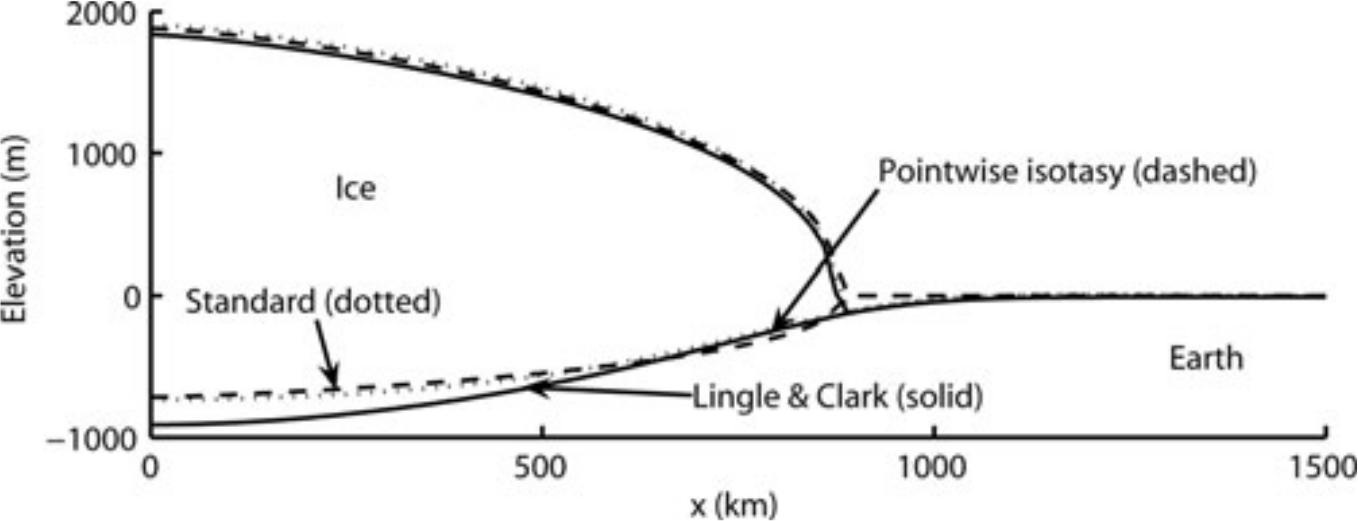
\includegraphics[width=0.75\textwidth]{photos/earthcompare}
\end{center}
\end{frame}


\begin{frame}{omitted models 4: numerical Stokes equations}

\begin{itemize}
\item the Stokes model itselfcan be solved numerically
  \begin{itemize}
  \item[$\circ$] no shallow assumptions!
  \item[$\circ$] but many more equations and unknowns than SIA, SSA, hybrids, Blatter, \dots
  \end{itemize}
\item requires \emph{explicit} accounting for
  \begin{itemize}
  \item[$\circ$] incompressibility $=$ a constraint on the flow
  \item[$\circ$] pressure $=$ a Lagrange multiplier for that constraint
  \end{itemize} 
\item very tough scalability issues:  can you afford the loss of resolution?  loss of long-time runs?
\item all of the success so far is at a smaller scale (e.g.~below)
\end{itemize}

\begin{columns}
\begin{column}{0.45\textwidth}
\scriptsize
Figure 7 in [Maxwell and others, 2008]\nocite{Maxwelletal2008}: \emph{Athabasca Glacier:  (a) modeled velocity contour lines ($\text{m}\,\text{a}^{-1}$); (b) contour lines derived from measurements [Raymond, 1971]\nocite{Raymond1971}}
\end{column}
\begin{column}{0.6\textwidth}
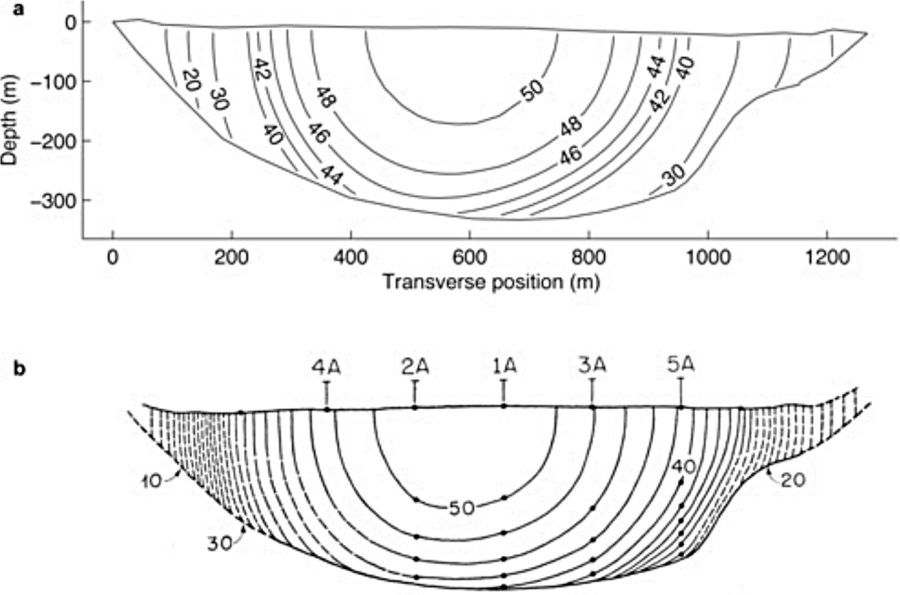
\includegraphics[width=0.75\textwidth]{photos/athabasca_cross}
\end{column}
\end{columns}
\end{frame}


\begin{frame}{omitted models 5: ``higher-order'' schemes}

\begin{itemize}
\item both the SIA and the SSA are derived by small-parameter arguments from the Stokes equations, so \dots
\item is there a \emph{common shallow antecedent model}?
\item Schoof and Hindmarsh [2009]\nocite{SchoofHindmarsh} answer:
  \begin{itemize}
  \item[$\circ$] \emph{yes}, the Blatter [1995]\nocite{Blatter} model is  intermediate between the Stokes stress balance and both the SIA and SSA
  \end{itemize}
\end{itemize}

\begin{center}
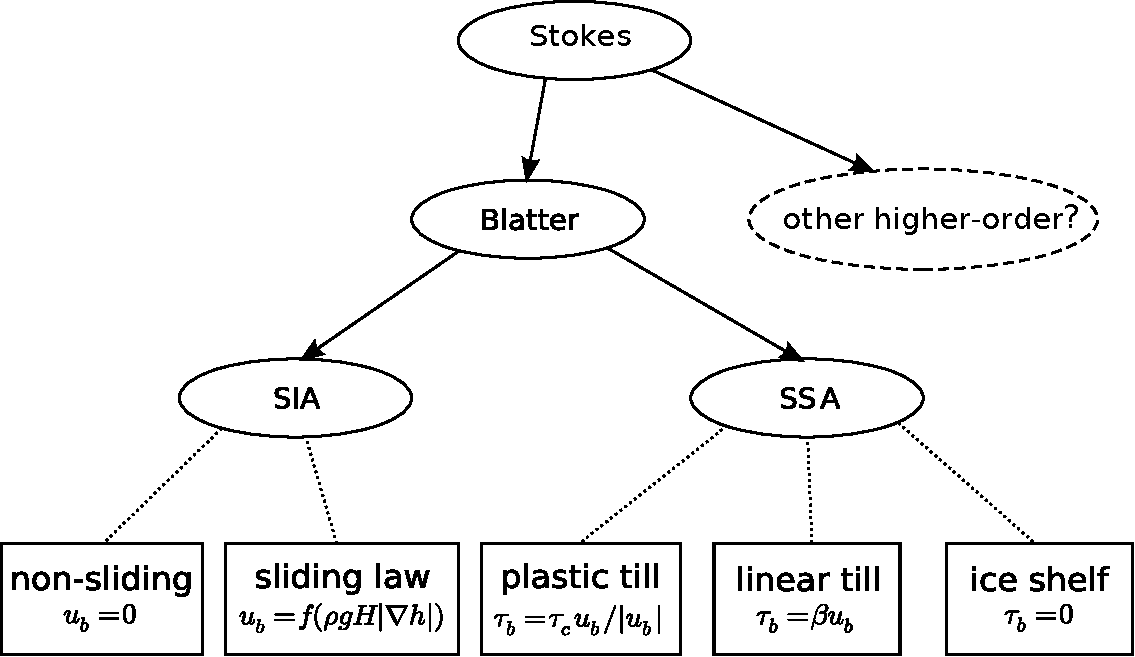
\includegraphics[width=0.7\textwidth]{photos/hierarchy}
\end{center}
\end{frame}
